\chapter{Background}
\lhead{\emph{Background}}
This chapter presents an overview of topics which are either prerequisites for autonomous exploration and coverage behaviour presented in the later chapters, or provide alternative solutions to the questions we are uncovering of how a robot can choose to move and coordinate.

\section{Overview}
Autonomous robots are systems which sense, actuate, compute and communicate. Sensing can be an ability to see, feel, hear or even a combination of them. For example a bot with a Kinect sensor has the ability to see. Similarly a bump sensor or a laser scanner attached to a bot will power it up with the ability to feel the presence of the obstacles around it. Actuation in this case is the bots' ability to move in the world. the following are the important functions and capabilities an autonomous robot 
must possess over other types of robots as summarized in \cite{7},
\begin{itemize}
    \item Gain information about the operating environment.
    \item Work for an extended period of time without human intervention.
    \item Move itself throughout its operating environment without human assistance.
    \item Avoid situations that are harmful to people, property, or itself unless those are designed so.
\end{itemize}
\vspace{5em}
This chapter will cover the following topics,
% \par Pose estimation : What is the sensors position with respect to a global reference frame, and how is it updated with the motion model? The SLAM problem.

\par \textbf{Mapping} : The robot plans its motion and performs exploration using a global map. Given a pose estimate and sensor data at the position, how do we integrate it into a globally consistent map structure?

\par \textbf{Exploration} : The robot should extend its global frame such that it covers the entire given space. Given a map and a current pose, how do we take high level decisions like where should the robot move next to achieve the above? 

% \par \textbf{Motion planning}: How is the robot made to move across the environment expanding the horizons avoiding fixed and dynamic obstacles?

% \section{Pose estimation}
% Assuming the robot has an initial scan of its immediate environment, we need to locate the robot with respect to its initial pose. It has to maintain an internal estimate of its position and orientation in the world. The pose estimate for a robot confined to ground plane will have two transnational components and one rotational component,
% \begin{equation} 
%     \textbf{p} = [x,y,z, \theta_{r},\theta_p,\theta_y]^T
% \end{equation}
% where $\theta_{r}, \theta_{p}, \theta_{y}$ are the roll angle around the x-axis, pitch angle around the y-axis and yaw angle around the z-axis. These six degrees of freedom are often referred to as 6DoF. The following are some standard methods for such estimate.

% \subsection{Dead reckoning}
% In navigation, dead reckoning is the process of calculating one's current position by using a previously determined position, or fix, and advancing that position based upon known or estimated speeds over elapsed time and course\cite{19}. 

% \subsection{Laser scan matching}

% \subsection{Visual odometry}

\section{Mapping}
Mapping is one of the core competencies of truly autonomous robots\cite{25}. Acquiring maps with mobile robots can be challenging for a number of reasons according to \cite{25}. First, even under discrete approximations, such as grid approximation, maps can be described in $10^5$ or more variable, making it challenging to calculate the full posteriors considering such high dimensional space. Second, As the robot moves through the environment, it accumulates errors in odometry, making it gradually less certain of its location in the map. Having this localization challenge, mapping also gradually becomes tough, since the robot's position becomes uncertain - The SLAM problem.

\subsection{Map representations}
To express the process of generating measurements, we need to specify the environment in which a measurement is generated. A map of the environment is a list of objects in the environment and their locations. While a topological map is concerned with the connections between locations and stored in a graph-like structure, a metric map maintains a model of the environment in a geometric sense which corresponds more directly to the real world. We used an occupancy grid as our map representation since frontier exploration works well with a grid based mapping approaches. The following are some representations of metric maps.

\subsubsection{Point clouds}
Point cloud representation is one of the closest forms of representation to the actual surroundings. The range sensor detects points in space and are then transformed into a global coordinate frame. These are then added to an existing collection which forms the point cloud. An example of a point cloud is shown above in Fig. 2.1.  

\begin{figure*}
    \begin{subfigure}[b]{0.498\textwidth}
		\centering
		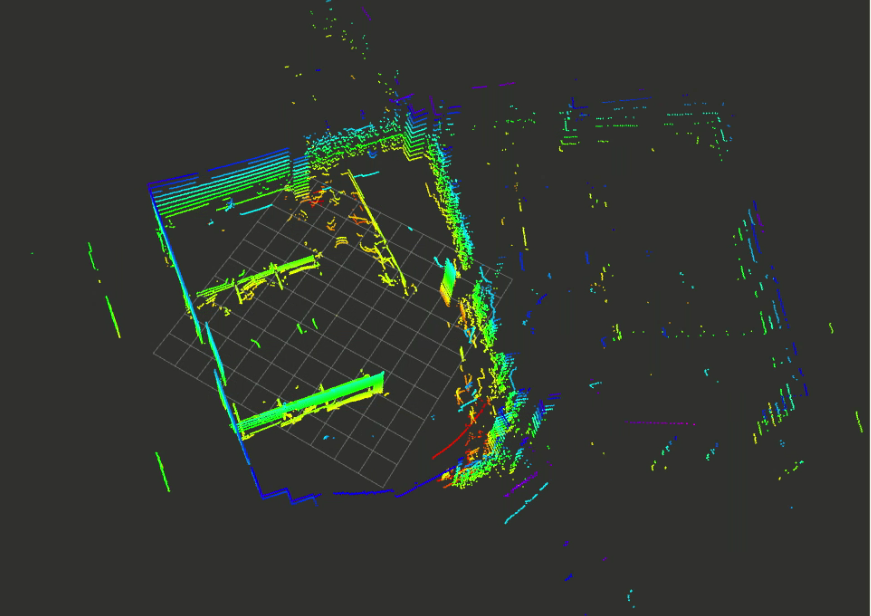
\includegraphics[width=\textwidth]{images/Symmetry_ppt.png}
		\label{subfig:a}
		\caption{}
		\vspace{2em}
	\end{subfigure}
	\begin{subfigure}[b]{0.498\textwidth}
	    \centering
		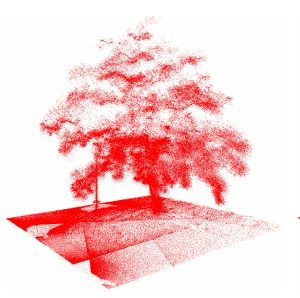
\includegraphics[width=\textwidth]{images/occupancytree.png}
		\label{subfig:b}
		\caption{}
	\end{subfigure}
    \caption{From left to right: Point cloud map representation using a VLP-16 LIDAR of the Drones Lab. A point cloud of a tree. Image from \cite{21}}
\end{figure*}

\subsubsection{Occupancy grids}
A classical map representation is known as occupancy grid map. Occupancy maps are location-based: They assign to each x-y coordinate a binary occupancy value which specifies whether or not a location is occupied with an object. Occupancy grid maps are great for mobile robot navigation\cite{25}. In other words, they make it easy to find paths through the unoccupied space. An occupancy grid is a quantified workspace with evenly spaced volumetric elements called voxels. Each voxel stores a probability of occupancy, i.e an estimate of whether there is an obstacle in that grid space. These probabilities are thresholded resulting in three values: \\
\noindent \textbf{Free} - This voxel or grid has been explored and is free of obstacles.\\
\textbf{Occupied} - This space has obstacles and robot senses that it cannot move into that space.\\
\textbf{Unknown} - The uncharted space that the robot needs to explore and get an idea of its occupancy.

\par These values can be represented using any random numbers but only that the nomenclature is to be persistent. The boundary upto which the robot can see or sense is called the horizon and the boundary which separates the free space with the unknown space is called the frontier. Each such cell which form the boundary is called a frontier cell. 

As per \cite{12}, the gold standard of an occupancy grid algorithm is to compute its posterior over the maps given data according to equation 2.1

\begin{equation} \label{eq:posterior}
    p(m|z_{1:t},x_{1:t})
\end{equation}

\noindent where \textit{m} is the map ${z_{1:t}}$ are the set of measurements up to time \textit{t}, and ${x_{1:t}}$ is the robot path, i.e the sequence of all its poses. ${m_i}$ refer to the index in each cell \textit{i}. Throughout this work $p(m_i = 100)$ is the probability that cell $m_i$ is occupied, and conversely $p(m_i = 0)$ is the probability it is empty. If $p(m_i = -1)$, it refers to the grid cell being an unknown cell. The posterior map probability given the sensor and the motion model is the product of the posteriors of each grid cell which is given by equation 2.2. 

% \begin{equation}
%     p(m|z_{1:t},x_{1:t})
% \end{equation}

% \noindent where $z_{1:t}$ is the set of all measurements until current time \textit{t}, and $x_{1:t}$ is the corresponding set of robot poses. the posterior of a map over the entire map can be given as the product of each grid cell,

\begin{equation}
    p(m|z_{1:t},x_{1:t}) = \prod_i{p(m_i|z_{1:t},x_{1:t})}
\end{equation}

Not only that occupancy grids are easy to construct and maintain, they work well in dynamic environments. Fig 2.2 represents an occupancy grid corresponding to the blue print of the environment which is inaccurate in certain places\cite{25}. If some data is corrupted by the presence of people; the occupancy grid map filters it out quite nicely. This makes occupancy grid maps much better suited for robot navigation than sets of scan endpoint data.

\begin{figure*}
    \begin{subfigure}[b]{0.498\textwidth}
		\centering
		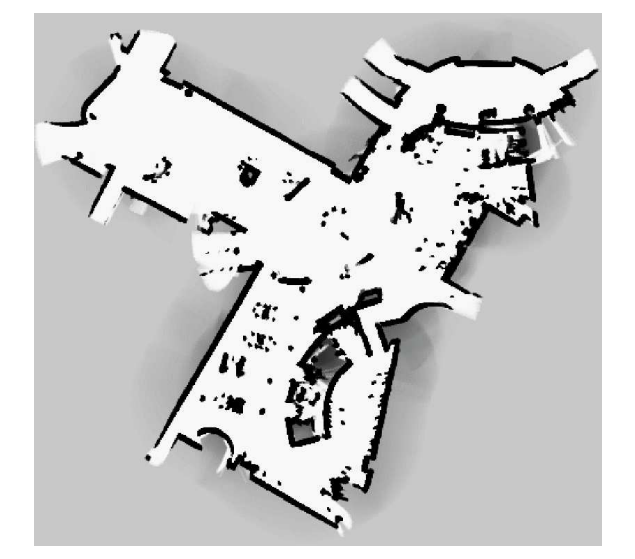
\includegraphics[width=\textwidth, height=0.75\textwidth]{images/occ1.png}
		\label{subfig:a}
		\caption{}
		\vspace{2em}
	\end{subfigure}
	\begin{subfigure}[b]{0.498\textwidth}
	    \centering
		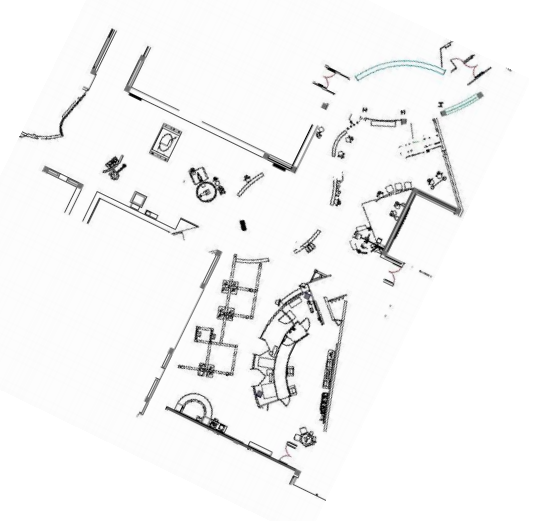
\includegraphics[width=\textwidth, height=0.75\textwidth]{images/occ2.png}
		\label{subfig:b}
		\caption{}
	\end{subfigure}
    \caption{(A)Occupancy grid map and (B)architectural blue-print of a large open exhibit space. Image from \cite{25}}
\end{figure*}

\subsubsection{2.5D Maps}
Handling full 3D occupancy grids can be challenging especially in can of limited computational resources. These limitations can be ameliorated when dealing with a robot constrained to the ground plane. 2.5D or elevation maps are a better alternatives to full 3D maps in such situations. These cells contain an estimate of the surface height at that position and can be sufficient for navigation and exploration\cite{12}\cite{13}. An example of a 2.5D map can be seen in Fig 2.3 above. The disadvantage of these map structures is that they are limited to a single height value at each cell, meaning environments containing multiple levels such as bridges or underpasses cannot be represented. Another disadvantage is their inability to represent free-space or unexplored regions numerically\cite{11}.  

\begin{figure}
    \centering
    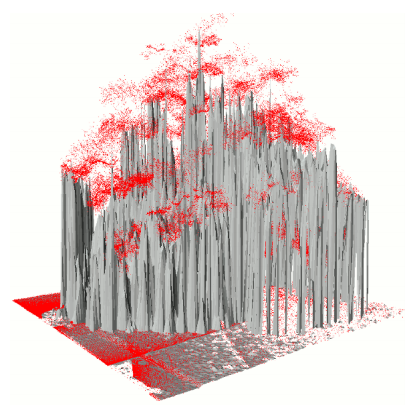
\includegraphics[width=0.5\textwidth]{images/25D.png}
    \caption{A 2.5D map of a tree. Image from \cite{21}}
    \label{fig:my_label}
\end{figure}

% % \section{Localization}
% \subsection{SLAM}
% \subsection{Path Planning}

\section{Autonomous Exploration and Coverage}
Exploration can be defined as maximizing the knowledge about the external world or simply the surroundings. Exploration has been a paramount problem in the field of robotics. A number of instances can be listed where exploration can help achieve a particular purpose like floor cleaning, detecting mines in an abandoned mine site, identifying humans stuck in disaster effected sites\cite{9}, interstellar explorations\cite{10}, etc. This in general, require the robotic device to be able to navigate. 
Autonomous exploration is a derivative of Coverage problem. Coverage simply implies the exploration performed has to cover the entire environment. Depending on the sensor(s) used, there are several applications like floor cleaning, lawn mowing, mine sweeping, search and rescue, etc. Exploration algorithm itself might not be complete and requires a coverage strategy to make it complete. Coverage is analogous to covering salesman problem, a variant of traveling salesman problem where the agent has to travel the neighborhood of the city as opposed to just visiting the city as in traveling salesman problem\cite{28}. 

\subsection{Traditional Coverage Approaches}

\begin{figure*}
    \begin{subfigure}[b]{0.498\textwidth}
		\centering
		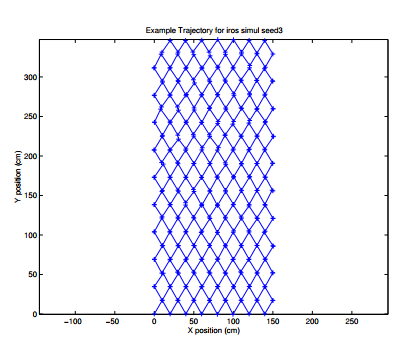
\includegraphics[width=0.85\textwidth, height=0.85\textwidth]{images/seed.png}
		\label{subfig:a}
		\caption{}
	\end{subfigure}
	\begin{subfigure}[b]{0.498\textwidth}
	    \centering
		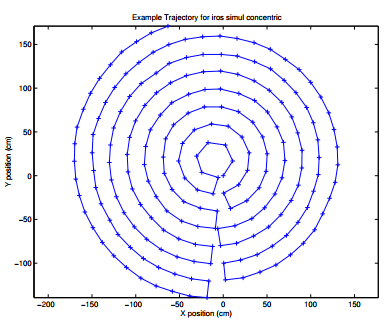
\includegraphics[width=0.85\textwidth, height=0.85\textwidth]{images/conc.png}
		\label{subfig:b}
		\caption{}
	\end{subfigure}
	\begin{subfigure}[b]{0.498\textwidth}
	    \centering
		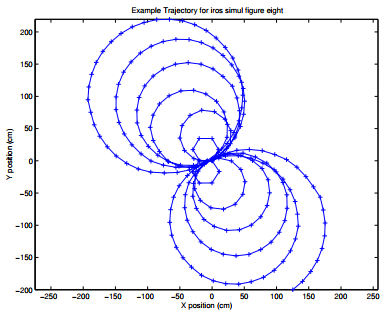
\includegraphics[width=0.85\textwidth, height=0.85\textwidth]{images/eight.png}
		\label{subfig:c}
		\caption{}
	\end{subfigure}
	\begin{subfigure}[b]{0.498\textwidth}
	    \centering
		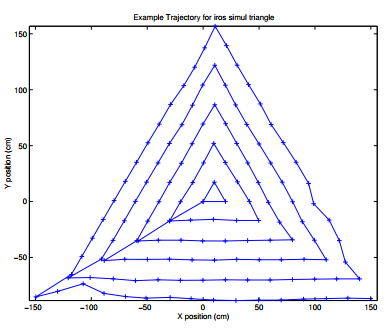
\includegraphics[width=0.85\textwidth, height=0.85\textwidth]{images/triangle.png}
		\label{subfig:d}
		\caption{}
	\end{subfigure}
	\begin{subfigure}[b]{0.498\textwidth}
	    \centering
		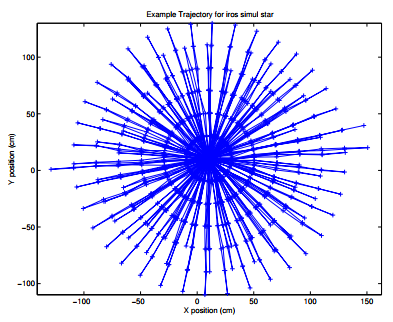
\includegraphics[width=0.85\textwidth, height=0.85\textwidth]{images/star.png}
		\label{subfig:e}
		\caption{}
	\end{subfigure}
    \caption{Different systematic approaches. Image from \cite{13}}
\end{figure*}

The early works in autonomous coverage can be classified into systematic or heuristic approaches and Non systematic approaches. Most of them suffer with atleast one drawback which includes incompleteness i.e they do not guarantee a successful exploration of the complete environment or they are probabilistically complete.

\textbf{Systematic approaches}: These approaches make the robot move in pre-defined patterns such that it unlocks new poses in the environment thereby exploring it.

\textbf{Non Systematic Approaches}: These approaches either rely on a random number generator or classify spaces to identify free space and usually involve a start-goal scenario.

\subsection{Systematic Approaches}
These are a set of heuristic behaviours that robots exhibit such as going in concentric circles, following a wall or evading obstacles\cite{8}. A combination of such behaviors can make the robot capable of accomplishing complex tasks like exploration. A variety of exploration trajectories have been developed and tested both in terms of coverage time as well as robot localization while executing the heuristic behavior. Some of them are described below\cite{26},

\noindent \textbf{Seed Spreader}: The robot follows a seed-spreader pattern through the environment\cite{27} as shown in Fig 2.4 (A).\\
\noindent \textbf{Concentric Circles}: The robot from its starting point goes in concentric circles reversing the direction for alternating circles as shown in Fig 2.4 (B).\\ 
\noindent\textbf{Figure Eight}: Similar to concentric circles, the robot traces them in a series of growing figure-eights, bringing the robot close to its starting point with each pass like shown in Fig 2.4 (C).\\ \noindent \textbf{Triangle}: The robot traces concentric equilateral triangular patterns shown in Fig 2.4 (D).\\ 
\noindent \textbf{Star}: This pattern makes the robot visit the starting point at each pass. The robot projects itself linearly and retraces the route only repeating it with a uniform difference in orientation at each pass. Fig 2.4 (E) shows the star pattern.\\

All the above strategies are proven to be either incomplete or probabilistically complete. The graph shown in Fig 2.5 shows the exploration efficiency plotted based on the images\/time step\cite{26}.

\begin{figure}
    \centering
    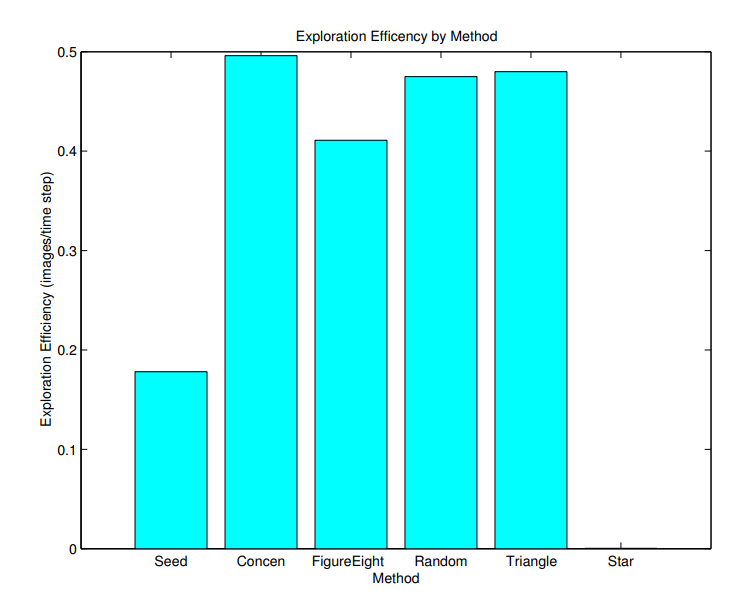
\includegraphics[width=0.75\textwidth]{images/expoeff.png}
    \caption{Evaluation of heuristic approaches discussed in Section 2.3.2}
    \label{fig:my_label}
\end{figure}

\subsection{Non Systematic Approaches}
These approaches do not follow a particular pattern or a heuristic and the trajectories covered are mostly unpredictable. The robot follows a formulation in order to pick its next move. The following are some non systematic approaches described.

\subsubsection{Random Approaches}
In this approach the robot selects a random pose with a threshold distance from itself. If it is unoccupied, the robot moves to it and repeats the same. This method have the following drawbacks,
\begin{itemize}
    \item The robot might end up picking already explored areas rendering the approach inefficient.
    \item Assuming the robot would pick all available poses in the environment, this approach is probabilistically complete.
\end{itemize}
A little smarter version is to select locations which are not explored. This would guarantee that the environment would be completely explored and hence makes the approach a complete one. These approaches are advantageous in terms of computational resources required but still prove to be inefficient in most cases when compared to other approaches such as frontier exploration.

\subsubsection{Frontier exploration}
A number of algorithms have being proposed for autonomous explorations. Frontier based exploration is one old and naive technique which is proved complete. This algorithm frees the robot to explore unknown spaces without the knowledge of prior data of obstacles in the given space. Frontier based exploration usually operate on grid maps. Unlike in other geometrical feature detection based maps like point or line maps, these maps distinguish between free, previously unexplored regions as shown in the Fig 2.6. The idea of frontier based exploration strategies is to guide the robot to the frontiers or boundaries between cells known to be free and cells for which no information is available\cite{25}. 

\begin{figure}
    \centering
    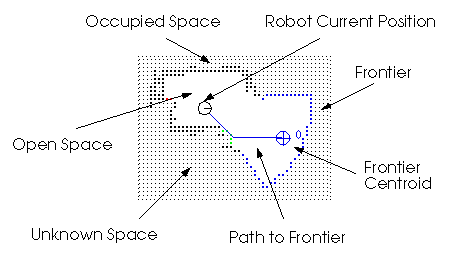
\includegraphics[width=0.75\textwidth]{images/frontier1.png}
    \caption{Imaging representing types of cells classified on an occupancy grid for frontier exploration}
    \label{fig:my_label}
\end{figure}

\subsection{Information gain exploration}
The above problem can be reduced to finding the next frontier which is logically considered to be the closest. This implies that the amount of information assigned or acquired at any frontier is the same. A better approach in finding the next poses which maximize expected uncertainty reduction. We implemented this approach for the comparative results in Chapter 4. 

\subsubsection{Entropy}
In information theory the measure of the information in a probability distribution \textit{p(x)} is the entropy \textit{$H_p(x)$} and is given by
\begin{equation}
    H_p(x) = - p(x)logp(x)dx
\end{equation}
Entropy is the measure of uncertainty associated with a random variable. $H_p(x)$ is maximal for a uniform distribution and this intuitively means that uncertainty is highest when all outcomes are equally likely. $H_p(x)$ decreases when $p(x)$ peaks and reaches zero when the outcome of the random trial is certain.

\subsubsection{Information gain}
The decrease in entropy between successive measurements is defined as the information gain \textit{I}. In the context of exploration this means that the difference in entropy at \textit{t+1} and at \textit{t} measures the information gained. Mathematically \textit{I} for a single voxel\/cell in an occupancy grid can be given by
\begin{equation}
    I(m_i|z_i) = H(p(m_i)) - H(p'(m_i|z_t))
\end{equation}
where, $p'(m_i|z_t)$ is the updated probability for the cell $m_i$ after updating the cell with a new measurement $z_i$ through the sensor model. The inverse sensor model allows us to estimate the information gain which we could expect if we were to move to a hypothetical new pose. This can be possible by ray-tracing through the occupancy grid, tracking the cells through which the ray passes. We follow a simple yet efficient method to measure the information gain by counting the number of unknown cells around each given frontier cell in a considerable radius.

\subsection{Cellular Decomposition}
These methods are developed to overcome the drawbacks of the above discussed approaches which are incomplete or probabilistically complete. All coverage approaches these days, that provide provable guarantee of completeness, use cellular decomposition\cite{35}. Three major classifications of cellular decomposition are approximate cellular decomposition which work on grid based representation of the free space, semi-approximate cellular decomposition which partially discretize the space and exact cellular decomposition is dividing the space into non intersecting regions.

\subsubsection{Approximate cellular decomposition}
This is a fine-grid representation where the union of all the cells only approximates the environment\cite{35}. In general, each cell in the grid is the size of robot's footprint which implies the cell is covered if the robot visits it. Complete coverage is achieved when all cells in the decomposition are visited. Zelinsky et al\cite{36} used conventional wavefront algorithm to achieve complete coverage. The wavefront algorithm initially assigns 0 to the goal, 1 to all of its neighbours and the remaining unmarked cells are labeled with a 2. This process is continued until the wavefront crosses the start and the robot uses a gradient descent on this numeric potential function\cite{37} to find a path.

\subsubsection{Semi-Approximate cellular decomposition}
Hert and Lumelsky developed a coverage algorithm that relies in a partial discretization of space where cells are fixed in width but the floor can have any shape\cite{38}\cite{39}. The robot can start at an arbitrary location in the map and perform zigzags along parallel straight lines. The smaller uncovered areas called inlets are detected by the robot and covered immediately in a depth-first order. The algorithm requires that the robot remember points at which it enters and exits inlets it covers assuring that each inlet is covered only once. 

\begin{figure}
    \centering
    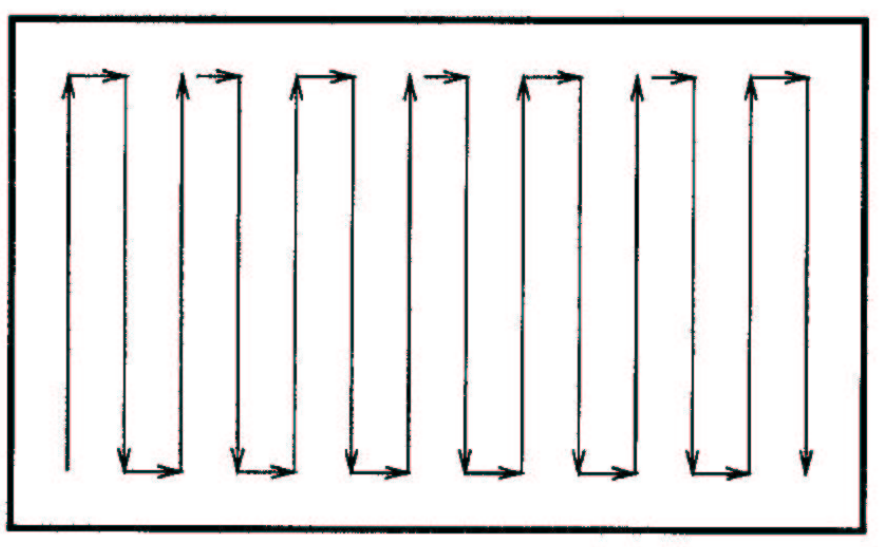
\includegraphics[width=0.5\textwidth]{images/bostrephroden.png}
    \caption{lawn mower trajectory: back and forth motions}
    \label{fig:my_label}
\end{figure}

\subsubsection{Exact cellular decomposition}
An exact cellular decomposition is the set of non-intersecting regions called cells, whose union fills the target environment\cite{35}. The robot can cover each cell using simple back-and-forth motions, reducing the coverage problem to motion planning problem.
Trapezoidal decomposition\cite{40} is a popular example of exact cellular decomposition technique where the free space is decomposed into trapezoidal cells. Each such cell is covered with simple back and forth motion shown in Fig 2.7. Coverage is achieved by visiting each cell in the adjacency graph. 
Boustrophedon decomposition is an extension to trapezoidal decomposition where many such trapezoidal cells can be merged such that no obstacle is in the robots path. Choset and Pignon\cite{35} developed this technique wherein new cells are added of the back-and-forth motion is obstructed by an obstacle and if not two cells are merged back into one cell as shown in Fig 2.8. 

\par All of the above techniques are proven to complete and neither of them require aprior information about the map. The weakness of these techniques would be their dependence on the grid resolution of the world. In order to perform complete coverage online, most techniques requires the robot to store information about the partially explored environment and perform additional computation to avoid edge cases such as revisiting a covered space. The disadvantage is that the complexity scales with the environment.  
% \subsubsection{Potential fields}
% \subsubsection{Graph methods}

\begin{figure}
    \centering
    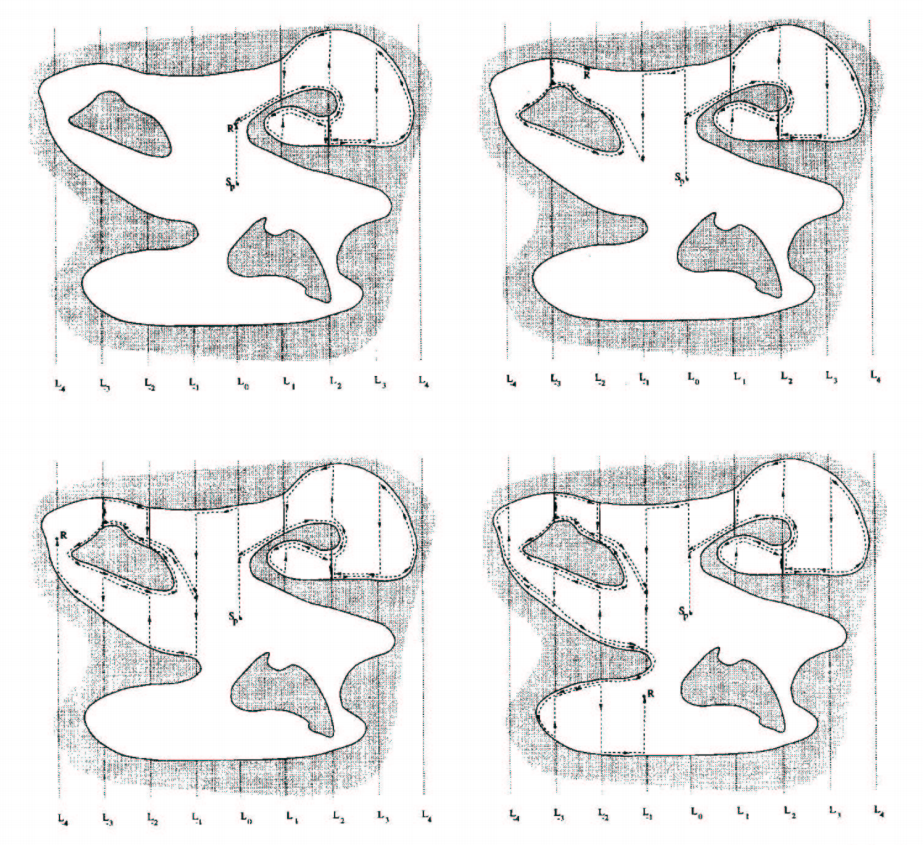
\includegraphics[width=\textwidth]{images/semiapproximate.png}
    \caption{A robot path using semi-approximate cellular decomposition in a map with islands and inlets. Images from \cite{35}}
    \label{fig:my_label}
\end{figure}

\section{Multi-Robot Coverage}
To reap the benefit of scaling efficiency with number of robots, multi robot exploration has been extensively researched in robotics community. The primary idea of using multiple robots is to improve coverage time. Though using multiple robots is advantageous, it does come with a set of challenge. The following are the prerequisites:
\begin{itemize}
    \item Communication network between robots for coordination
    \item Path planning utilities for robots
    \item Coordination schemes: Centralized or distributed
    \item Coverage strategy
\end{itemize}

\subsection{Coordination Control}
Typically two schemes for coordination between robots are available:

\noindent \textbf{Centralized Coordination scheme}:
Using a central coordinator, generally one of the robots or a separate system is deployed to help communication possible between robots. This master robot or system assigns the navigation tasks to the robots and make sure all the components are working properly. The benefit of using such a scheme is that its easier to implement but has a probability of single point failure. In other words, if the central node fails, the entire system crashes.

\noindent \textbf{Decentralized or distributed control}:
As the name indicates, in this scheme the robots are self reliant and take their own navigation decisions. These robots are connected using a Wi-Fi network and communicate their respective positions and progress. Though this scheme does not suffer from single point failure, the communication traffic in the network plays a role in deciding the algorithms efficiency.

\subsection{Multi robot Coverage Strategies}
There are various coverage strategies available for collaborative robotics. The most popular of them are summarized below\cite{43}. 

\subsubsection{Potential Fields}
Robots follow a gradient descent in a fine-grid two dimensional map. Work by Howard et al proposed a multi robot coverage approach where robots repel each other until an equilibrium is reached. Since equilibrium is not analogous to complete coverage, this approach suffers from incompleteness. An improved version of this approach is that an overlapping potential field is introduced where robots repel from the obstacles and attract to unexplored space. Even this suffers with the disadvantage of of robots getting stuck in local minima\cite{45}. 

\subsubsection{Graph methods}
In this approach the map is represented in the form of a graph where edges represent hallways and nodes represent the intersections in the environment. Once the graph is formed complete coverage is achieved using traveling salesman problem\cite{46}.  .

\subsubsection{Frontier methods}
Frontier exploration used for single robot has been developed for multiple robots in different variants where the primary problem to be solved is frontier allocation. Frontiers are nothing but a boundaries which separate the empty space from unknown space. This method works on grid maps than point or line maps\cite{25}. The occupancy grid which represent the environment is discretized into three values representing three spaces: free, occupied or unknown\cite{17}. 
Rogers et al proposed a centralized scheme of allocating frontiers to multiple robots where one of the robots is the master. The master both detects and allocates frontiers to the fellow robots in a greedy manner. In other words, each frontier allocated to the robot is the nearest to it. Many approaches have been developed like \cite{46}\cite{47}. All these approaches require frontiers to be identified and clustered. We use image processing to identify frontiers in this work. Other method include wavefront detection where a wave front is propagated towards the goal. Each strategy has its own advantage, disadvantages and requirements. One should be selecting them based on the sensor payload and type of environments to explore.